%\documentclass{acm_proc_article-sp} UNCOMMENT FOR NO PAGE NUMBERS (doesn't extend/reduce document length)
\documentclass[preprint]{acm_proc_article-sp} %Remove preprint for camera-ready 
\pagenumbering{arabic} % Remove for camera-ready

\usepackage{graphicx}
\usepackage{amsmath}
\usepackage{float}
\usepackage{natbib}
\usepackage{url}
\usepackage{amssymb}

% our packages
\usepackage{algorithmic}    % AA pseudocode
\usepackage{algorithm}      % AA pseudoocode
\usepackage{multirow}       % results tables
\usepackage{array}          % results tables
\newcolumntype{C}[1]{>{\centering\let\newline\\\arraybackslash\hspace{0pt}}m{#1}} % results tables
\usepackage{etoolbox}       % shrug

\makeatletter
\patchcmd{\maketitle}{\@copyrightspace}{}{}{}
\makeatother

\begin{document}
\title{Analysis of Adaptive Aggressive on the\\
Bristol Stock Exchange}
\numberofauthors{3} 
\author{
  \alignauthor
    Rupert Bedford\\
    \email{rb9281@bristol.ac.uk}
  \alignauthor
    Max Robinson\\
    \email{mr9388@bristol.ac.uk}
  \alignauthor
    Jonathan Simmonds
    \email{js9721@bristol.ac.uk}
}
\date{7 December 2012}

\maketitle
\begin{abstract}
As robot traders are now commonplace within the financial environment
\cite{nyse_press}, we
wished to evaluate various algorithmic trading strategies. Our primary focus was
the  Adaptive Aggressive algorithm considered to be one of the
best in the field \cite{AA_thesis}. We experimented with different parameters for the algorithm
and then evaluated the performance of it against other common traders,
including ZIP and ZIC \cite{ZIP_paper1}, finding that it conclusively
outperformed these approaches.\\
\end{abstract}

\section{Introduction} \label{sec:introduction}
% OWNER: Rupert
% - What is automated trading (history)
% - What our goal was

An automated trader is an algorithm that automatically places trading orders on
an electronic market. In 2012 on the New York Stock Exchange program trading accounted for between 
30\% and 40\% of the trade volume \cite{nyse_press}.
A trader receives buy and sell orders from customers where an order consists of a price the customer 
wants to trade at and the volume they want to trade.
The trader makes money through the margin between the order price and the price they trade at.
A trading strategy has to balance the profit margins with the change of completing a trade to maximise profit.

In a double auction the bids and asks determine the price of the commodity.
When a bid equals or exceeds a seller's ask the bid is accepted and the trade
occurs. Experiments have shown  that the prices in the market will
 converge on the price equilibrium in a number of market
environments \cite{smith_1962}.

IBM published a paper in 2001 that showed that their Modified Gjerstad Dickhaut (MGD) trading strategy and
Dave Cliff's ZIP were able to outperform human traders \cite{ibm_human}.
Algorithmic strategies are able to react more quickly to changing market
conditions and combine information from multiple sources.

In this paper we experiment with different trading strategies for the
continuous double auction.
We implement the Adaptive Aggressive strategy \cite{AA_thesis} and compare its performance 
with other adaptive algorithms and simpler traders.\\



\section{Environment} \label{sec:environment}
\subsection{BSE} \label{sec:BSE}
The Bristol Stock Exchange (BSE) is a virtual trading environment for the
continuous double auction. Each trader has access to Level 2 market data which
includes the individual buy and sell orders (the limit order book). The
environment is simpler than a real exchange as traders only buy or sell one
unit of a single commodity at a time. Traders can also take as long as they
need to respond to market events and submit orders. BSE includes 5 traders: Giveaway, ZIC, Shaver, Sniper and ZIP.

Traders have access to the limit order book which contains the outstanding
shouts made in the market. The limit order book is anonymised so the identity
of the trader who made each shout is unknown. At each simulation time step a
random trader is asked to make a shout. If the maximum bid in the market
exceeds or equals the minimum ask a trade occurs. Each trader is updated with
any orders or trades that have occurred since the last update.

Some trading algorithms require more depth in the order book. The MGD algorithm needs to be able to match trades with
outstanding orders to build up the accepted and rejected order histories.
This is covered in more detail in Section \ref{sec:traders_GDV}. The
other traders in our experiments only need Level 1 data
(bid-high and ask-low).

Traders are assigned orders to a given supply and demand schedule. BSE supports three methods of price 
generation: \emph{Fixed}, \emph{Random} and \emph{Jittered}. \emph{Fixed} price generation maintains 
a constant difference between orders when they are sorted by price. The \emph{Random} mode generates 
orders uniformly at random in a given range while \emph{Jittered} mode is similar to \emph{Fixed} 
except that it adds a small amount of noise --- making it closer to a real world exchange. There are 
also three options for determining when orders are submitted to traders: \emph{Drip Fixed}, 
\emph{Drip Jittered} and \emph{Drip Poission}. With \emph{Drip Fixed} orders arrive at a fixed 
interval, \emph{Drip Jittered} is similar but with a small amount of added noise and finally 
\emph{Drip Poisson} models the arrival of orders as a Poisson process.\\



\subsection{Traders} \label{sec:traders}
\subsubsection{ZIC} \label{sec:traders_ZIC}
% OWER: Jonny
% - 
The Zero Intelligence (ZI) agents were first proposed in 1993 \cite{ZIC_paper} and are trading agents 
which have `zero intelligence' --- they simply make offers randomly between the maximum and minimum 
allowed market price. Zero Intelligence Constrained (ZIC) traders are marginally more intelligent as 
they make offers randomly between the worst offer ever seen and their limit price --- preventing them 
from losing money on trades.

ZIC trader's random behaviour, which appears to exhibit human-like characteristics \cite[p.~1]{ZIP_paper1}, 
makes them perfect as a control to test our algorithm's performance against. We used the 
implementation of ZIC provided in the BSE (Section \ref{sec:BSE}).\\



\subsubsection{ZIP} \label{sec:traders_ZIP}
% OWNER: Jonny
% - What was significant --- key points
% - Advantages/disadvantages
Zero-Intelligence-Plus (ZIP) traders were invented in 1997 and designed to improve on ZIC traders 
(Section \ref{sec:traders_ZIC}) \cite{ZIP_paper1}. They make use of a simple learning mechanism which 
allows them to adjust their profit margin in response to other completed trades on the market --- thus reacting to 
current market conditions. In turn this defines their current offer(s). This algorithm allows surprisingly complex behaviour with a 
minimal performance cost.

The key parameters in the algorithm are the learning rate, $\beta$ --- which represents how quickly 
the trader reacts to market change; and the `momentum', $\gamma$ --- which represents how market 
volatility is smoothed over. More accurately, the learning rate controls how quickly the algorithm 
moves towards its current target price while the momentum controls how quickly the algorithm changes 
its profit margin over time.

The change in price at subsequent time steps can be defined mathematically for a single given trader as:
\begin{equation}
    \Delta(t) = \beta \cdot ( \tau(t) - p(t))
    \label{eqn:change_in_price}
\end{equation}
where $\tau(t)$ is your target price and $p(t)$ is your current offer on the market (or `shout').

The change in profit margin at subsequent time steps can then be defined as:
\begin{equation}
    \Gamma(t) = \gamma \cdot \Gamma(t-1) + (1 - \gamma) \cdot \Delta(t)
    \label{eqn:change_in_margin}
\end{equation}

This allows the new margin to be calculated:
\begin{equation}
    \mu(t) = \frac{p(t) + \Gamma(t)}{l} - 1
    \label{eqn:new_margin}
\end{equation}
where $l$ is your limit price.

Finally the new price can be calculated by:
\begin{equation}
    p(t+1) = l \cdot (1 + \mu(t))
    \label{eqn:new_price}
\end{equation}

We used the implementation of the ZIP algorithm provided in the BSE (Section \ref{sec:BSE}).\\



\subsubsection{GD variants} \label{sec:traders_GDV}
% OWNER: Rupert
% - Shavers / Sniper / XKCD, etc.
% - MGD anonymised data (see BSE paragraph 2)
% - We implemented it but couldn't do a full implementation

The Gjerstad Dickhaut (GD) trading strategy was invented by Steven Gjerstad and John Dickhaut in 
their 1998 paper \emph{Price Formation in Double Auctions} \cite{gd}.
GD works by building a belief function of whether a bid at a particular price
will be accepted by a seller.
The buyer then aims to maximise their profit through a combination of margin
and chance of trading.
The belief values are formed based on observed trades and outstanding shouts.
The GD strategy makes some simple assumptions, such as: if a bid was rejected a
lower bid will also be rejected since it will be less attractive to a seller.
The results of the experiments showed that GD has a higher price efficiency than ZIC.
The price efficiency is the margin divided by the maximum theoretical margin
(difference between limit and price equilibrium).
They also showed that GD was able to cope with changing supply and demand
conditions.

The GD belief function for a seller is given by:
\begin{equation}
  f(p) = \frac{\text{AAG}(p) + \text{BG}(p)}{\text{AAG}(p) + \text{BG}(p) +
  \text{UAL}(p)}
\end{equation}
where $\text{AAG}(p)$ is the number of accepted asks in the history window $\geq p$.
$\text{BG}(p)$ is the number of bids $\geq p$. $\text{UAL}(p)$ is the number of unaccepted asks $\leq p$.

Modified Gjerstad Dickhaut (MGD) \cite{mgd} is a version of GD that
is better suited to volatile conditions that can occur at the start of a
session where there is very little information about accepted and rejected
orders.
An MGD agent remembers the highest and lowest prices from the last session.
An MGD buyer will then set the belief function to 1 for all prices above the
lowest price and to 0 for all prices below the lowest price.
MGD is also able to hold multiple units.

GDX \cite{gdx} is a Dynamic Programming based variant of GD.
GDX uses the same belief function as GD but uses Dynamic Programming to
maximise the long term reward instead of the short term reward.
Dynamic Programming is used to compute optimal policies in Markov Decision
Problems.
The emphasis placed between short and long term rewards can be controlled using
the discount value ($\gamma$).
$\gamma = 0$ will result in the same behaviour as the standard GD strategy
(short-term reward) while $\gamma = 1$ will cause GDX to maximise the long term
reward.
However setting $\gamma$ close to 1 will cause GDX to always wait for a better
deal and thus not make any trades.
Under certain market environments GDX is able to outperform
both GD and ZIP.
With a $\gamma$ between 0.75 and 0.85 GDX always outperforms GD.
GDX is more flexible than GD and can handle multiple goods although
optimisations are needed to keep the state space tractable.\\



\subsubsection{Other traders}
The giveaway trader submits orders at its limit price so never makes any profit
or loss unless it is given a new order whilst it has an outstanding shout in
the market. The shaver trader submits a shout one price unit better (for the
other party) than the current best shout. The sniper trader gets increasingly
aggressive the closer it is to the end of the session. The aggressiveness
controls the amount it is willing to improve the current best shout.\\



\subsection{Adaptive Aggressive traders} \label{sec:AA}
% OWNER: Max
% - ???
The main focus of our experiments was the Adaptive Aggressive trader created by
Vytelingum in 2006 \cite{AA_thesis}. The Adaptive Aggressive algorithm relies on the principal that you can be in
two different states. One where you trade closer to your limit
price, with an increased chance of trading but lower profit per trade. The other where you
trade further from your limit price, decreasing the likelihood of making a
trade but increasing the amount of profit you will make upon a successful trade.

The Adaptive Aggressive algorithm maintains an aggressiveness value ($r$) which
determines how close to your limit price you will be trading. A completely
aggressive buyer ($r = 1$) will bid at their limit price whilst a completely
passive buyer ($r = -1$) will bid at the minimum market price (\$1 on the BSE).\\



\subsubsection{Price equilibrium estimator}
One of the key features that most trading algorithms rely on is the ability to
estimate the equilibrium price of the market. For this we used the following
equation which estimates the market equilibrium price based on the $N$ most
recent transactions, known as a weighted moving average.
\begin{equation}
    \hat p^* = \frac{\sum^T_{i=T-N+1}w_ip_i}{\sum^T_{i=T-N+1}w_i}\\
    \label{eqn:equilibrium_estimator}
\end{equation}
where $w_T = 1$ and $w_{i-1} = \lambda w_i$.

The $w_i$ weights the transactions so more weight is given to more recent
transactions. A lower $\lambda$ value will increase the emphasis on more recent trades. We set the 
value of $\lambda$ to 0.9 which was the value recommended in the original paper 
\cite[p.~100]{AA_thesis}. We also investigated the effect of different values of $\lambda$ on the algorithm's 
performance, the results of which are detailed in Section \ref{sec:calibration_lambda}.\\



\subsubsection{Price estimation} \label{sec:AA_price_estimation}
% OWNER: Max
% - Graph of all trades with projected price equilibrium
% - MEGA GRAPH
The Adaptive Aggressive algorithm calculates the price of its shout by
computing a target price ($\tau$) which is dependent upon
the state of the market. However, before we can go into detail, we must define
two concepts: intra-marginal and extra marginal traders. An intra-marginal trader bids above the
equilibrium if they are a buyer (or asks below the equilibrium if they are a
seller) whereas an extra-marginal trader will never trade above the
equilibrium if they are a buyer (or below the equilibrium if they are a
seller).

Whether our trader is acting in an intra-marginal or extra-marginal capacity
will depend upon the limit price for our order. For a buyer we act as an intra-marginal trader if we 
have a limit price above the equilibrium (or below the equilibrium for a seller) otherwise we act as 
an extra-marginal trader. This difference is illustrated in Figure \ref{fig:r_price}, where we plot 
our target price ($\tau$) against the aggressiveness ($r$) using the different trading strategies. In 
this example the buyer's extra-marginal limit is 5 with an intra-marginal limit of 15 (and vice versa 
for the seller). For an intra-marginal trader there is an inflection point at the price equilibrium 
(10 in our example).

\begin{figure}[H]
\centering
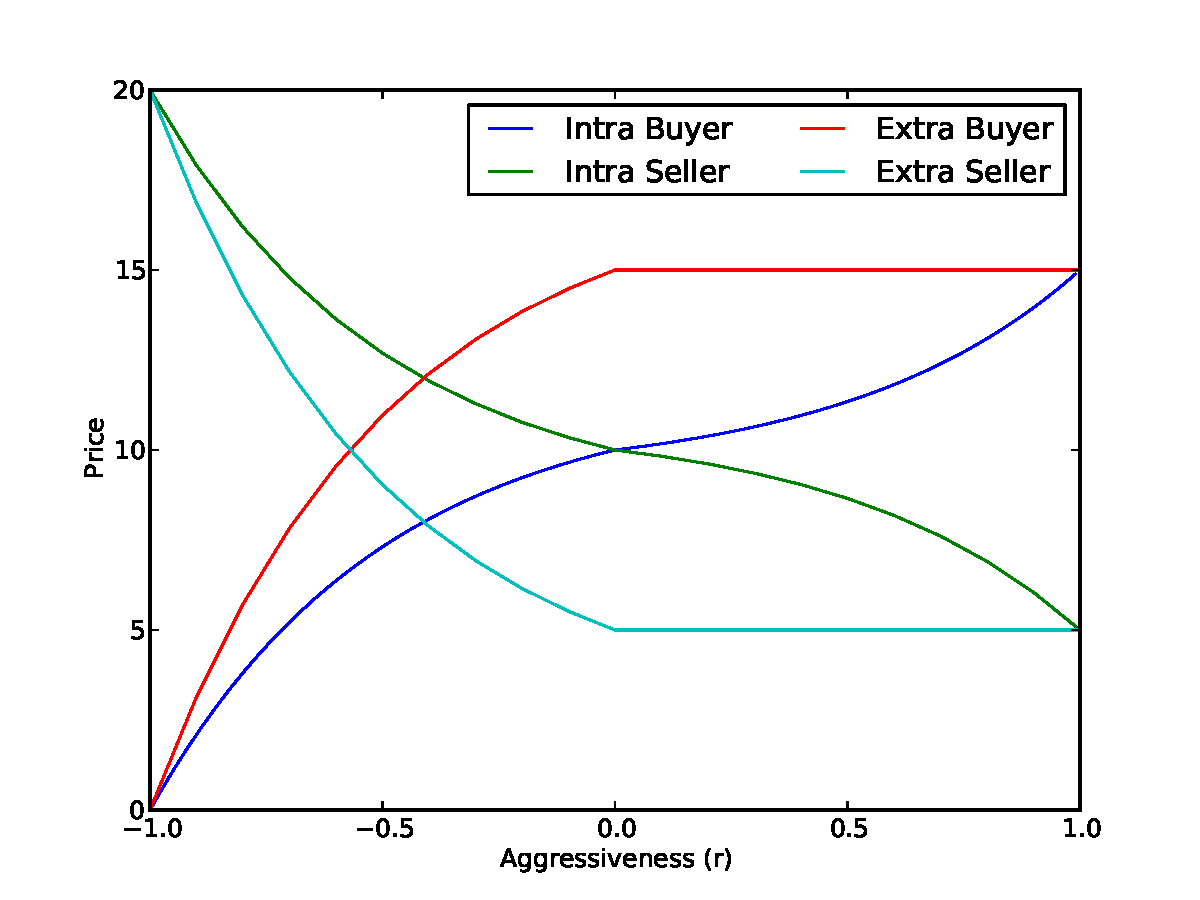
\includegraphics[width=\columnwidth]{graphs_and_stats/graph_r.pdf}
\caption{Graph showing relationship between target price and aggressiveness for different trading strategies.}
\label{fig:r_price}
\end{figure}

The price that we then submit will depend upon which capacity we are acting
under, based on the following equations.

\textbf{Intra-marginal buyer}
\begin{equation}
    \tau =
    \begin{cases}
        \hat{p}^*(1- \frac{e^{-r\theta}-1}{e^{\theta}-1}) &  \text{if r} \in (-1,0)  \\
        \hat{p}^* + (l_i-\hat{p}^*)(\frac{e^{r\theta}-1}{e^\theta-1}) & \text{if r} \in (0,1)
    \end{cases}
    \label{eqn:intrabuyer}
\end{equation}
where $\theta$ (Section \ref{sec:AA_long_term_learning}) measures the volatility of the
market, $l_i$ is the limit price for the buyer, and $\hat{p}^*$ is the estimator of the
equilibrium price.

\textbf{Extra-marginal buyer}
\begin{equation}
    \tau =
    \begin{cases}
        l_i(1-\frac{e^{-r\theta}-1}{e^\theta-1}) &  \text{if r} \in (-1,0)  \\
        l_i & \text{if r} \in (0,1)
    \end{cases}
    \label{eqn:extrabuyer}
\end{equation}

\textbf{Intra-marginal seller}
\begin{equation}
    \tau =
    \begin{cases}
        \hat{p}^* + (\text{MAX}-\hat{p}^*)( \frac{e^{-r\theta}-1}{e^{\theta}-1}) &  \text{if r} \in (-1,0)  \\
        c_j + (\hat{p}^*-c_j)(1-\frac{e^{r\theta}-1}{e^\theta-1}) & \text{if r} \in (0,1)
    \end{cases}
    \label{eqn:intraseller}
\end{equation}
where MAX is the maximum price that can be submitted to the market and $c_j$ is
the limit price for the seller.

\textbf{Extra-marginal seller}
\begin{equation}
    \tau =
    \begin{cases}
        c_j + (\text{MAX}-c_j)(1-\frac{e^{-r\theta}-1}{e^\theta-1}) &  \text{if r} \in (-1,0)  \\
        c_j & \text{if r} \in (0,1)
    \end{cases}
    \label{eqn:extraseller}
\end{equation}

In the paper \cite{AA_thesis} an extra variable ($\underline \theta$) is used in addition to $\theta$ 
ensuring the first derivatives of the equations are continuous. However, we found that just using 
$\theta$ was sufficiently accurate and greatly simplified the above equations.

One of the equations is selected to determine the ideal price that we aim to
trade at. The following rules are then used to determine the actual shout
that we will make when asked to submit a new order. The $o_{bid}$ and $o_{ask}$
represent the highest bid and lowest ask on the market that have
not yet been accepted. The value of $\eta$ is set as a parameter and reflects
how quickly we converge on our estimated price (higher $\eta$ causes slower convergence). We investigated the effect of different $\eta$ values on profits as detailed in Section \ref{sec:calibration_eta}.

%\textbf{Bidding rules for buyer:}
\begin{algorithm}[H]
    \caption{Bidding rules for buyer}
    \begin{algorithmic}
        \IF{$l_i \leq o_{bid}$}
            \STATE submit no bid (market transacting above our limit).
        \ELSE
            \STATE submit bid given by $\textstyle o_{bid} + \frac{\textstyle \tau - o_{bid}}{\textstyle \eta}$.
        \ENDIF
    \end{algorithmic}
    \label{alg:bidding_rules_buyer}
\end{algorithm}

%\textbf{Bidding rules for seller:}
\begin{algorithm}[H]
    \caption{Bidding rules for seller}
    \begin{algorithmic}
        \IF{$c_j \geq o_{ask}$}
            \STATE submit no ask (market transacting below our limit).
        \ELSE
            \STATE submit ask given by $\textstyle o_{ask} - \frac{\textstyle o_{ask}-\tau}{\textstyle \eta}$.
        \ENDIF
    \end{algorithmic}
    \label{alg:bidding_rules_seller}
\end{algorithm}

Since these all require an existing bid on the market, there are different
rules used to determine which shout to make if we are the first
trader selected. These rules can be found in the Adaptive Aggressive
paper \cite[p.~32]{AA_paper}.

Initially when we ran our algorithm we found that it was occasionally making a
loss upon receiving a new order from the scheduler containing a different limit
price. This was because our last shout had been submitted using
the limit price from the previous order (which may now be outside the range
we are allowed to trade within). We therefore added additional logic to detect a new order enabling 
us to react appropriately. Since on the Bristol Stock Exchange it is not possible to withdraw a shout, 
if it was found that the new order contained a limit that was outside of our trading range, we 
cleared the previous bid using a stub.\\



\subsubsection{Short term learning} \label{sec:AA_short_term_learning}
% OWNER: Max
% - Graphs - r vs price equilibrium.
The aggressiveness of the Adaptive Aggressive algorithm is updated at every
time step using Equation \ref{eqn:update_aggressive} based on the following rules:

\begin{algorithm}[H]
  \caption{Learning rules for buyer}
  \begin{algorithmic}
    \IF{trade occurs at price $q$}
        \IF{$\tau \geq q$}
            \STATE be less aggressive (our price too high).
        \ELSE
            \STATE be more aggressive (our price too low).
        \ENDIF
    \ELSIF{ $\tau \leq o_{bid}$ }
        \STATE be more aggressive (our price too low).
    \ENDIF
  \end{algorithmic}
  \label{alg:learning_rules_buyer}
\end{algorithm}

\begin{algorithm}[H]
  \caption{Learning rules for seller}
  \begin{algorithmic}
    \IF{trade occurs at price $q$}
        \IF{$\tau \leq q$}
            \STATE be less aggressive (our price too low).
        \ELSE
            \STATE be more aggressive (our price too high).
        \ENDIF
    \ELSIF{ $\tau \geq o_{bid}$ }
        \STATE be more aggressive (our price too high).
    \ENDIF
  \end{algorithmic}
  \label{alg:learning_rules_seller}
\end{algorithm}

To update our aggressiveness we first calculate our target aggressiveness:
\begin{equation}
    \delta(t) = (1 \pm \lambda_r) \cdot r_{shout} \pm \lambda_a
\end{equation}
We then move towards it from our original aggressiveness ($r$) at 
a rate determined by a constant ($\beta_1$):
\begin{equation}
    r(t+1) = r(t) + \beta_1 \cdot (\delta(t) - r(t))
  \label{eqn:update_aggressive}
\end{equation}
The effect that different values of $\beta_1$ have on performance is explored in Section \ref{sec:calibration_beta}.

The function $\delta(t)$ is primarily dependent on the value of $r_{shout}$, the aggressiveness that 
would give a target price of the best outstanding shout when used in the equations found in Section 
\ref{sec:AA_price_estimation}. The value of $r_{shout}$ is calculated by reversing the aforementioned 
equations, as seen in the example given in Equation \ref{eqn:reverse_intra_buyer} which calculates 
$r_{shout}$ from the reverse of the intra-marginal buyer.
\begin{equation}
r_{shout}=
\begin{cases}
 -\ln\left(\frac{ \left( 1-\frac{\tau}{\hat p^*} \right) \left( e^\theta-1 \right) + 1}{\theta}\right) & \tau
< \hat p^*\\
\ln\left( \frac{ \left( e^\theta -1 \right) \left( \frac{\tau - \hat p^*}{l_i - \hat p^*} + 1 \right)
}{\theta} \right)&
\textstyle{otherwise}
\end{cases}
\label{eqn:reverse_intra_buyer}
\end{equation}

When we wish to become more aggressive we set our target aggressiveness slightly higher than the
value of $r_{shout}$, conversely slightly lower when we wish to become less aggressive. This is accomplished by
setting the sign of $\lambda_r$ and $\lambda_a$ where positive $\lambda$ values increase aggressiveness,
 whereas negative $\lambda$ values decrease aggressiveness.
The actual values of $\lambda_r$ and $\lambda_a$ represent the relative and absolute difference from $r_{shout}$
respectively. The absolute change exists to prevent $r$ from never being able
to update from a value of 0.\\



\subsubsection{Long term learning} \label{sec:AA_long_term_learning}
% OWNER: Max
% - theta
The Adaptive Aggressive algorithm takes into account the volatility of the market, tracked using the
$\alpha$ value, and adjusts its behaviour accordingly by altering the relationship between aggressiveness and price.

The  value of $\alpha$ (see Equation \ref{eqn:alpha}) is calculated
by looking at the variance of the last $N$ trades around the market equilibrium.
If the majority of trades are close to the equilibrium price then we are in
a stable market and vice versa. The smallest and largest expected market volatility are represented 
by $\alpha_{min}$ and $\alpha_{max}$ (these are initialised to 0.02 and 0.15 respectively).
\begin{equation}
  \alpha = \frac{\sqrt{\frac 1 N \sum^T_{i=T-N+1}(p_i-\hat p^*)^2}}{\hat p^*}
  \label{eqn:alpha}
\end{equation}
This long term learning is accomplished by incorporating a variable ($\theta$) which is updated every
timestep to move towards $\theta^*(\alpha)$ at a rate determined by $\beta_2$ (see Equation \ref{eqn:update_theta}).
The larger the value of $\beta_2$ the faster we converge towards $\theta^*$. We initially set the 
learning rate to 0.5, however we also investigated different values of $\beta_2$, as discussed in 
Section \ref{sec:calibration_beta}.
\begin{equation}
  \theta(t+1)=\theta(t)+\beta_2(\theta^*(\alpha)-\theta_t)
  \label{eqn:update_theta}
\end{equation}
The value of $\theta^*(\alpha)$ represents the value of $\theta$ that will allow us to act optimally in a
market with a volatility of $\alpha$. A high value of $\theta$ is desirable in a stable market.
\begin{equation}
  \theta^*(\alpha) = (\theta_{max}-\theta_{min})
  \left(\frac{1-e^{\gamma\left(\frac{(\alpha-\alpha_{min})}{(\alpha_{max}
  -\alpha_{min})}-1\right)}}{1-e^{-\gamma}}\right)
  \label{thetastar}
\end{equation}
This value of $\theta^*$ is scaled with
respect to a minimum and maximum value, $\theta_{min}$ and $\theta_{max}$, constants that are hard coded into the
function (we used -8 and 2 respectively).

\begin{figure}[H]
  \centering
  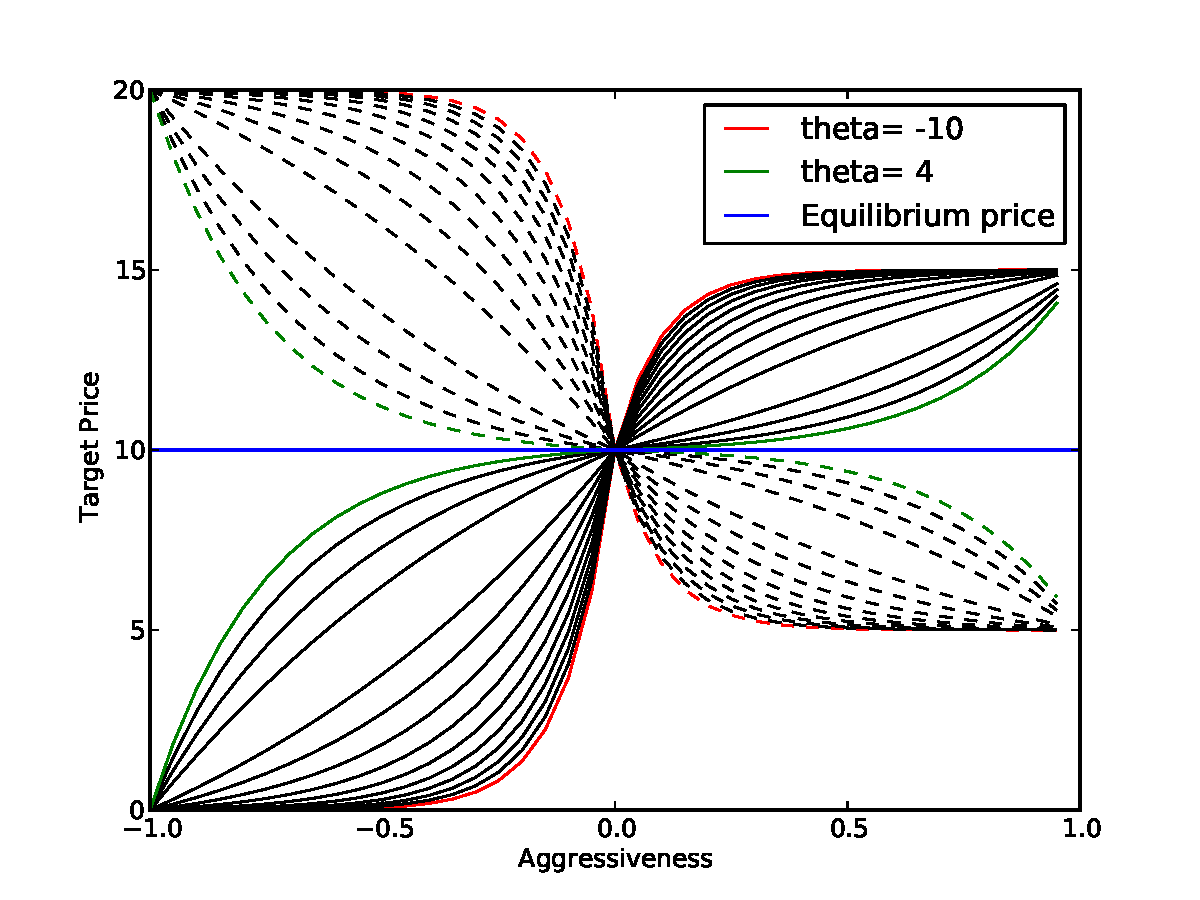
\includegraphics[width=\columnwidth]{graphs_and_stats/graph_thetas.pdf}
  \caption{How different $\theta$ values affect the target price calculations.}
  \label{fig:theta}
\end{figure}

The $\theta$ affects the degree to which changing the aggressiveness moves the
target price away from the equilibrium. A high value of $\theta$ means that a
relatively large change in aggressiveness will only result in a small move away from
the equilibrium price. This is illustrated in Figure \ref{fig:theta}, when
$\theta=4$ for $r \in (-0.5, 0.5)$ the price stays very close
to the equilibrium.\\



\section{Calibration} \label{sec:calibration}
% OWNER: Group
% - $\beta_1$, $\beta_2$, $\gamma$, $\eta$
% - potential to compare statistically?
Adaptive Aggressive has a number of tunable parameters. In this Section we
explore these and their effect on the algorithm's performance in the market.\\


\subsection{$\eta$ parameter} \label{sec:calibration_eta}
The $\eta$ value in the Adaptive Aggressive bidding function determines how
quickly the shout price moves from the best shout in the market towards the
calculated target price. A higher value of $\eta$ will increase the time taken
to converge on the target price, making the trader slower to react to market
events. 

We tested various values of $\eta$ across 3,000 market sessions in
order to test the effect on Adaptive Aggressive's performance, including $\eta
= 3$, the value recommended in the original thesis \cite{AA_thesis}.
\begin{table}[H]
  \centering
  \begin{tabular}{ | c | c | }
    \hline
    \textbf{$\eta$ value} & \textbf{Average finishing balance (3 dp.)} \\
    \hline
        1 & 125.317 \\
        3 & 138.971 \\
        5 & 140.538 \\
        10 &  139.560\\
        100 & 119.576 \\
        1000 & 117.996 \\
    \hline \hline
        ZIC & 85.040 \\
        ZIP & 124.753 \\
    \hline
  \end{tabular}
  \caption{Difference in finishing balance with respect to change in $\eta$.}
  \label{tbl:eta_results}
\end{table}
As is illustrated in Table \ref{tbl:eta_results}, as long as $\eta$ is
within reasonable limits, between 3 and 10 in our example, it does not
significantly impact the performance. However, setting $\eta$ too low would cause outlier trades to have a significant
impact on our shout price. Conversely setting $\eta$ too high causes the
algorithm to be slow to react. Both of these are backed up by data in Table
\ref{tbl:eta_results}.\\



\subsection{$\beta_1$ and $\beta_2$ parameters} \label{sec:calibration_beta}

The constants $\beta_1$ and $\beta_2$ are the learning rates for aggressiveness
and $\theta$ respectively.  We update our aggressiveness and $\theta$ values
more often than in the original Adaptive Aggressive paper \cite{AA_thesis}.
Whilst this is advantageous as it allows us to adapt to rapidly changing market
conditions, it means that our learning rates have to be comparatively lower to
avoid the algorithm effectively learning immediately. Learning rates that are very high, or very low, should have an
adverse effect on the performance of the trader. We ran tests over
4,000 market sessions with various different values of $\beta_1$ and
$\beta_2$, the results are shown in Table \ref{tbl:beta_results}.  The average
profit made by the Adaptive Aggressive algorithm did not appear to be significantly affected by the $\beta_2$ value. Variation in $\beta_1$ had more of an effect; setting the value of $\beta_1$ to zero gave a marked drop in performance.
This is because the aggressiveness will be constant and our algorithm will not
be able to adapt to changing market conditions. With a value of zero for $\beta_2$,
$\theta$ becomes constant although this does not appear to have a significant effect on profits. 
\begin{table}[H]
  \centering
  \begin{tabular}{ | c | C{2.7cm} | C{2.7cm} | }
    \hline
    \multirow{2}{*}{\textbf{Value ($v$)}} & \multicolumn{2}{ c | }{\textbf{Average finishing balance (3 dp.)}} \\
    & $\beta_1 = v, ~ \beta_2 = 0.5$ & $\beta_1 = 0.5, ~ \beta_2 = v$ \\
    \hline
        0.00 & 112.970 & 128.071 \\
        0.01 & 124.706 & 128.212 \\
        0.02 & 125.680 & 128.157 \\
        0.03 & 126.911 & 128.366 \\
        0.04 & 127.360 & 128.177 \\
        0.05 & 127.744 & 128.088 \\
        0.06 & 127.607 & 128.308 \\
        0.07 & 127.770 & 128.000 \\
        0.08 & 128.672 & 128.100 \\
        0.09 & 128.827 & 128.173 \\
        0.10 & 128.839 & 128.903 \\
        0.20 & 129.402 & 129.287 \\
        0.30 & 129.097 & 129.376 \\
        0.40 & 128.766 & 129.344 \\
        0.50 & 129.228 & 129.081 \\
        0.60 & 129.510 & 129.187 \\
        0.70 & 129.023 & 128.947 \\
        0.80 & 129.384 & 129.144 \\
        0.90 & 129.480 & 129.405 \\
        1.00 & 129.357 & 129.368 \\
    \hline \hline
    ZIC & \multicolumn{2}{ c | }{ 89.030} \\
    ZIP & \multicolumn{2}{ c | }{117.461} \\
    \hline
  \end{tabular}
  \caption{Finishing balance with respect to change in $\beta_1$ and $\beta_2$ values.}
  \label{tbl:beta_results}
\end{table}



\subsection{$\lambda$ parameter} \label{sec:calibration_lambda}
The constant parameter $\lambda$ controls the weighting of prices in the trade history. The higher the $\lambda$ value the more weight will be given to older trades. We tested $\lambda$ values from $0$ to $1$ in $0.1$ increments over 8,000
market sessions to find their effect on our trader's
performance. We did not find any statistically significant difference between
the different values. 

\begin{table}[H]
  \centering
  \begin{tabular}{ | c | c | }
    \hline
    \textbf{$\lambda$ value} & \textbf{Average finishing balance (3 dp.)} \\
    \hline
        0.0 & 128.048 \\
        0.1 & 128.040 \\
        0.2 & 128.041 \\
        0.3 & 128.314 \\
        0.4 & 128.268 \\
        0.5 & 128.278 \\
        0.6 & 128.224 \\
        0.7 & 128.380 \\
        0.8 & 128.172 \\
        0.9 & 128.365 \\
        1.0 & 128.462 \\
    \hline \hline
        ZIC &  89.521 \\
        ZIP & 116.719 \\
    \hline
  \end{tabular}
  \caption{Difference in finishing balance with respect to change in $\lambda$.}
  \label{tbl:lambda_results}
\end{table}

\begin{figure}[H]
  \centering
  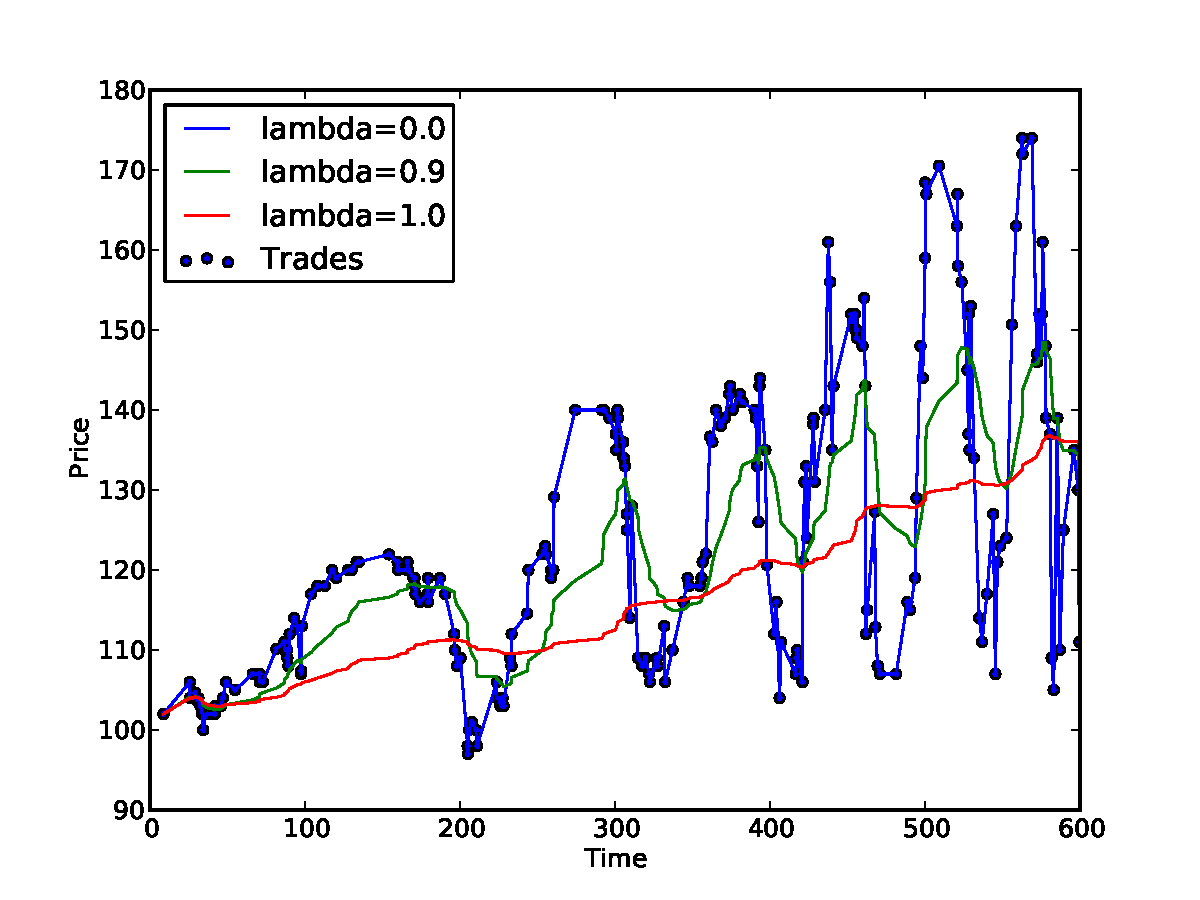
\includegraphics[width=\columnwidth]{graphs_and_stats/graph_equilibriums.pdf}
  \caption{The effect of the weighting value on the price equilibrium
  \label{fig:equilibrium}
  estimate.}
\end{figure}



\section{Evaluation} \label{sec:evaluation}
% OWNER: Group
% - Graph: Average balance over time
% - Statistical analysis - why you used a certain test
%   Ed's report: ``According to the conducted Wilcoxon-Mann-Whitney two-tailed rank-sum tests, the difference in the observed efficiencies is significant ($U = 2, N_1 = N_2 = 10, p < 0.0003$)."
% - Experiment with changing scheduler
% - Other graphs
In this section we compare the performance of the Adaptive Aggressive trader
with other traders as well as looking at how specific aspects of the Adaptive
Aggressive algorithm work in practice.\\


\subsection{Aggressiveness} \label{sec:evaluation_aggressiveness} 
The aggressiveness across a trading day is illustrated in Figure \ref{fig:avtime}.
In order to collect more data, we
increased the scheduler to distribute orders every five timesteps instead of
every thirty. This increases the number of trades in the market, giving us more
trading data to work with and allowing us to generate a far more accurate
estimate of the price equilibrium. This change only affects the data
represented in Figures \ref{fig:avtime} and \ref{fig:theta_v_time}.

One of the first conclusions we can draw from the graph is that our trader is
always playing an active role in the market ($r > 0$), trading above the market
equilibrium. This is because the market was set up to distribute orders with a
periodic nature. Therefore, each trader receives a similar limit price
resulting in a competitive market necessitating trades closer to the limit
price. 

At the start of the day, our trader has a lower aggressiveness value (close to
zero), this is because the trader lacks information about the market and
therefore adopts a more passive role to prevent selling far above the
equilibrium.

The dips in the aggressiveness correspond to the falling equilibrium price
where we can afford to trade further below our limit because the gap between
our limit price and the market equilibrium is increasing.


\begin{figure}[H] 
\centering
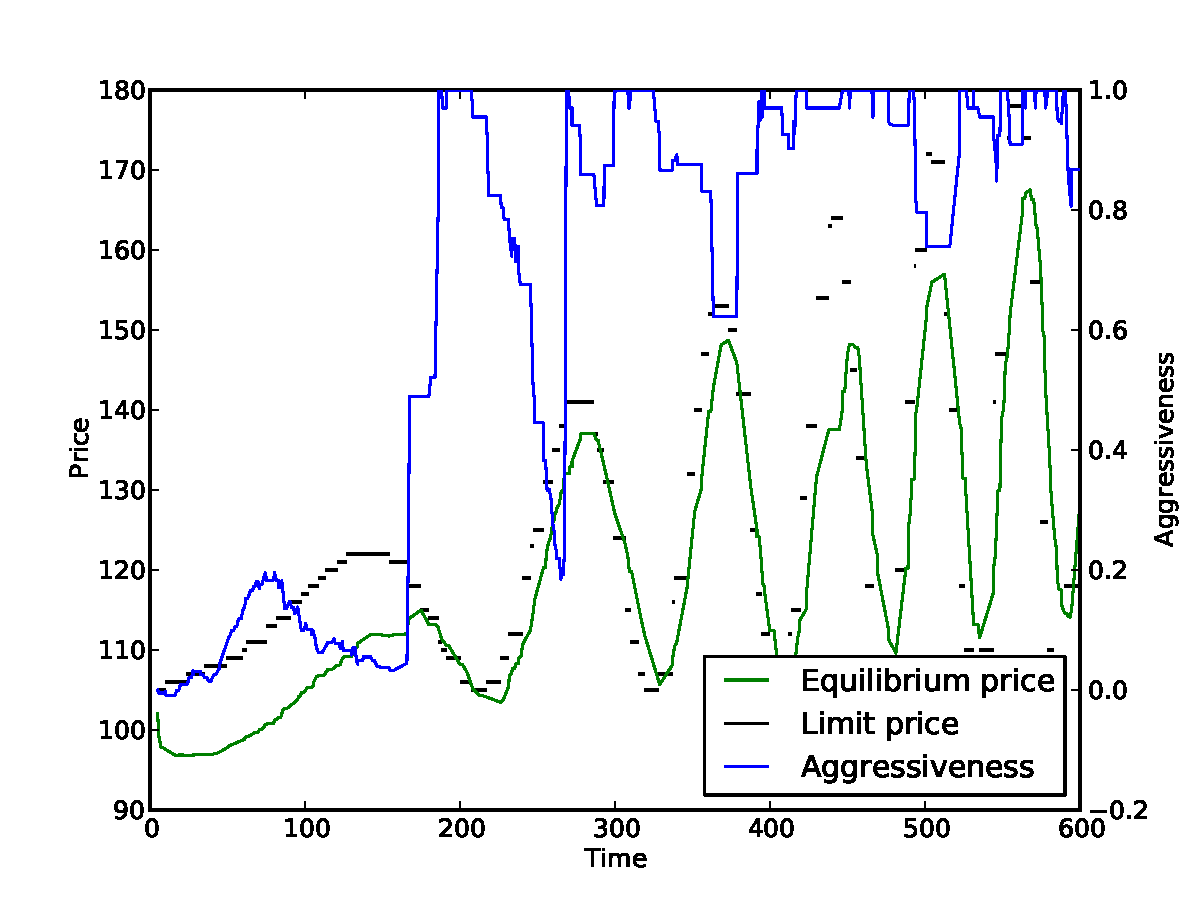
\includegraphics[width=\columnwidth]{graphs_and_stats/graph_aggressiveness_vs_price.pdf}
\caption{Aggressiveness and price equilibrium throughout a trading day for an AA
  buyer.}
  \label{fig:avtime}
\end{figure}



\subsection{Long term learning ($\theta$)} \label{sec:evaluation_theta}
Figure \ref{fig:theta_v_time} illustrates our value of $\theta$ throughout the
trading day. It peaks at the beginning of the market session when the market is
most stable then decreases as the market begins to oscillate.

The reason the $\theta$ value is unstable is due to the fact that at the
extremes of the sine wave all previous trades appear to be very far from the
current equilibrium estimate, resulting in the trader believing the market is
extremely volatile. On the other hand the slope represents a value where the
equilibrium price is closer to the average price in the trade history.
\begin{figure}[H]
  \centering
  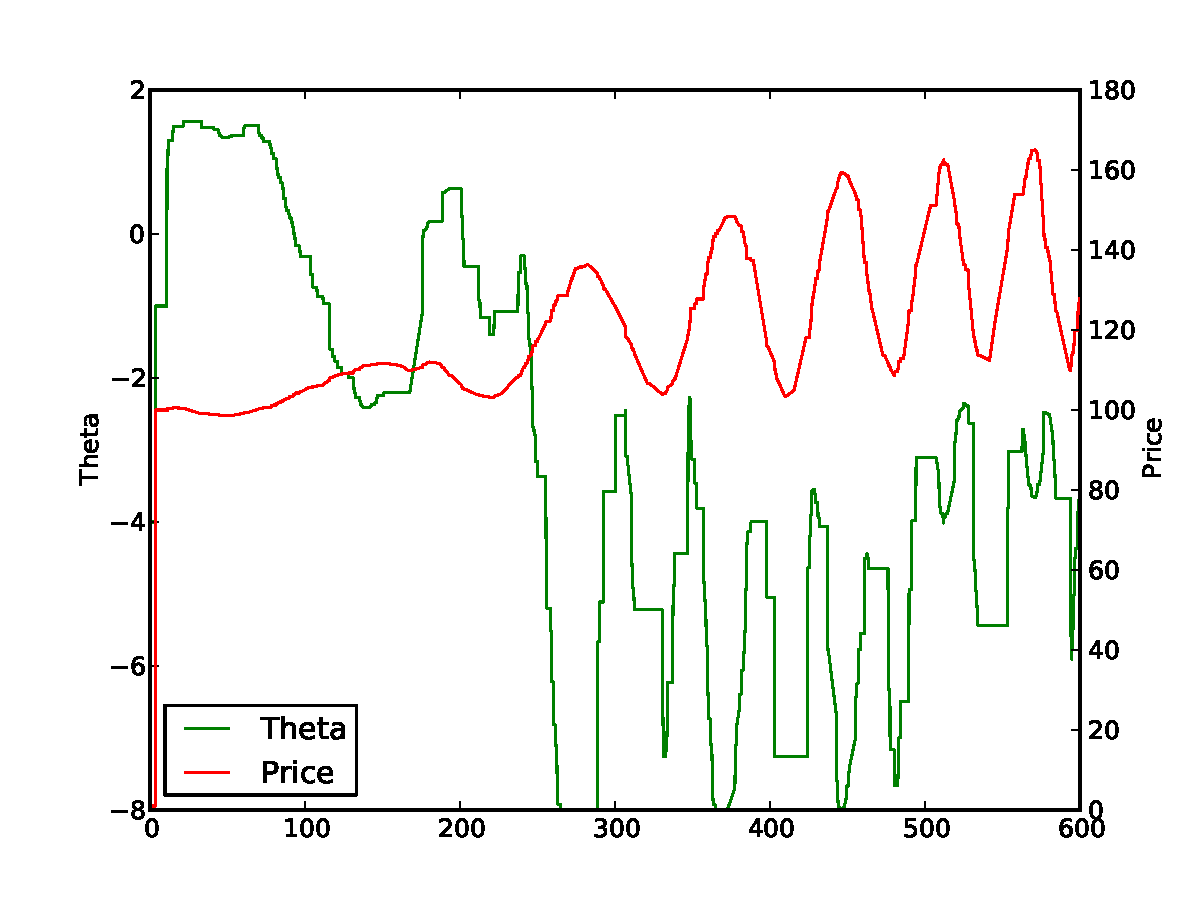
\includegraphics[width=\columnwidth]{graphs_and_stats/graph_theta_vs_time.pdf}
  \caption{How $\theta$ varies across a market day.}
  \label{fig:theta_v_time}
\end{figure}

\subsection{Comparison of traders using the sinusoidal order schedule}
\label{sec:eval_schedule}
In order to evaluate the performance of our Adaptive Aggressive trading
algorithm we ran 22,750 market sessions with different ratios of AA, SHVR, ZIC
and ZIP traders (half buyers, half sellers). For each ratio 50 market sessions
were run and the results are presented in Table \ref{tbl:results}. As
illustrated, we can see that the Adaptive Aggressive trader comprehensively outperformed all of the other
traders.

\begin{table}[H]
  \centering
  \begin{tabular}{ | c | C{2.5cm} | C{2.5cm} | }
    \hline
    \multirow{2}{*}{\textbf{Strategy}} & \multicolumn{2}{c|}{\textbf{Average
    finishing balance (3 dp.)}} \\
%    \cline{2-3}
%    & \vspace{0.05cm} Fixed & \vspace{0.05cm} Jittered \\
    & Fixed & Jittered \\
    \hline
    ZIC & 93.863 & 93.713 \\
    SHVR & 106.139 & 106.270  \\
    ZIP & 120.434 & 120.543 \\
    AA & 136.555 & 136.428 \\
    \hline
  \end{tabular}
  \caption{Average balances for different trading strategies.}
  \label{tbl:results}
\end{table}

The Wilcoxon signed-rank test was used to evaluate the significance of the
results. The null hypothesis is that the difference between the pairs of
traders is zero. For each trader paired with the Adaptive Aggressive trader we can reject
the null hypothesis ($p < 2.2 \cdot 10^{-308}$). The results using fixed and
jittered price generation were virtually identical.

\begin{figure}[H]
  \centering
  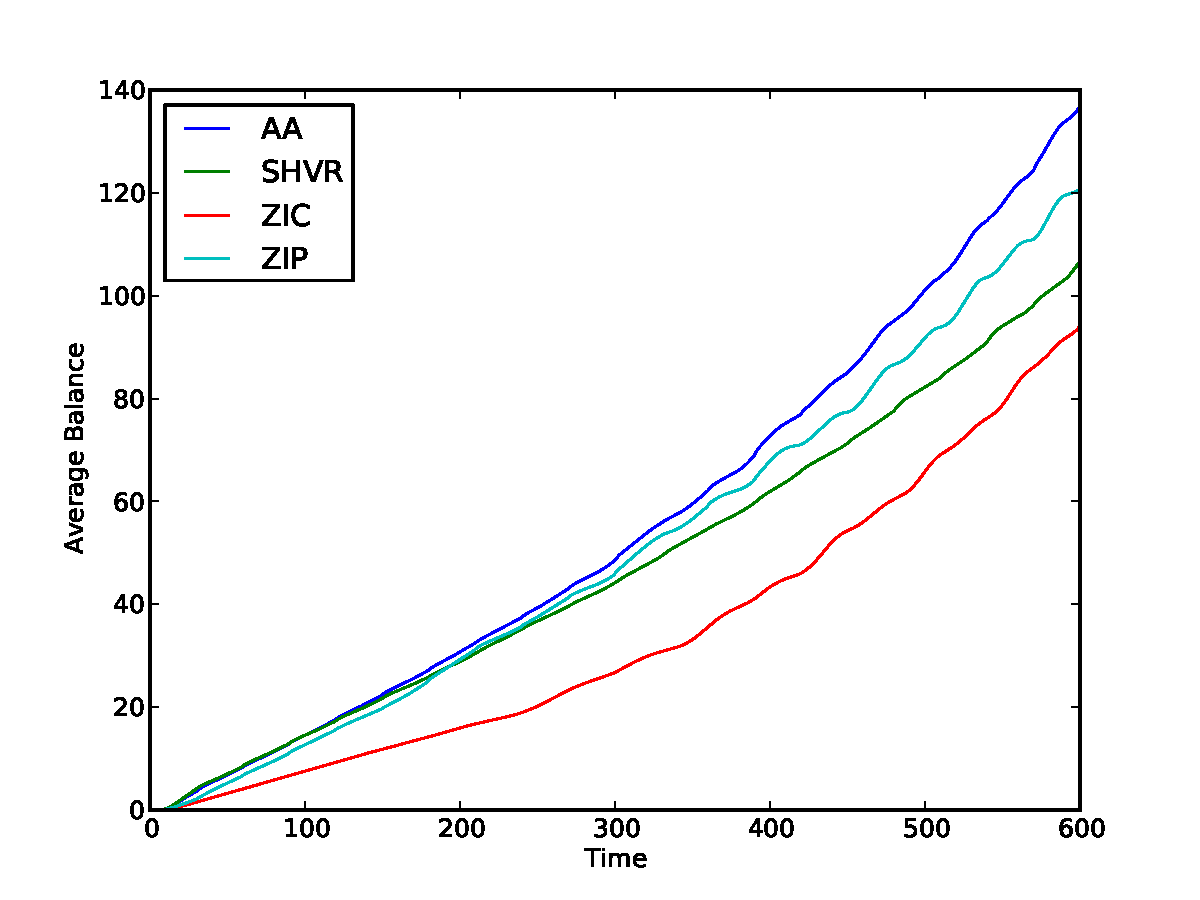
\includegraphics[width=\columnwidth]{graphs_and_stats/graph_average_balance_vs_time.pdf}
  \caption{Average balance over 22,750 trials.}
  \label{fig:average_balance_vs_time}
\end{figure}

Figure \ref{fig:average_balance_vs_time} graphs performance throughout a trading day and shows that the Adaptive Aggressive trader consistently
makes more profit.

We also compared how well the Adaptive Aggressive algorithm performed against
only ZIP across 10,000 market sessions. This was done to verify that the
Adaptive Aggressive algorithm is not just exploiting weaker traders which would
not exist in a real world competitive market. As is visible in Table
\ref{tbl:two_traders} with just two traders in the market the difference
between AA and ZIP is even more pronounced.
\begin{table}[H]
  \centering
  \begin{tabular}{ | c | c | }
    \hline
    Strategy & Average finishing balance (3 dp.) \\
    \hline
    ZIP & 110.006 \\
    AA & 136.378 \\
    \hline
  \end{tabular}
  \caption{Market session with just AA and ZIP traders.}
  \label{tbl:two_traders}
\end{table}

We ran the Wilcoxon signed-rank test on the values in Table
\ref{tbl:two_traders} which resulted in $p < 2.2 \cdot 10^{-308}$ which proves that AA is better than ZIP in this market. The Adaptive Aggressive
traders outperformed the ZIP traders 99.66\% of the time. Since ZIP performs worse it suggests that ZIP was reliant on trades with the
ZIC and SHVR traders.\\


\subsection{Comparison of traders using the disjoint order schedule}

We also ran an experiment comparing the performance of Adaptive Aggressive, ZIP
and ZIC traders, across 1,000 market sessions, using a different order schedule.
This divides the
market up into three phases each with a  different limit range. For each phase,
every trader receives a random limit from the respective range. The results of this
experiment can be seen in Table \ref{tbl:disjoint_market}.
\begin{table}[H]
  \centering
  \begin{tabular}{ | c | c | }
    \hline
    Strategy & Average finishing balance (3 dp.) \\
    \hline
    ZIC & 132.282 \\
    ZIP & 140.774 \\
    AA & 141.239 \\
    \hline
  \end{tabular}
  \caption{Market session with disjoint order schedule.}
  \label{tbl:disjoint_market}
\end{table}
In this experiment ZIP and Adaptive Aggressive had similar performance. We ran the
Wilcoxon signed-rank test with a significance threshold of 0.05 which concluded
that Adaptive Aggressive and ZIP were not significantly different. However,
since the ZIC trader was also relatively competitive, it suggests that this is
not an accurate representation of a real world market as ZIC is essentially random.\\

% TODO: Big graph of time and price

\section{Conclusion} \label{sec:conclusion}
% OWNER: Group
% - Thank you and good night
% - Hold for applause
In this paper, we wrote an implementation of the Adaptive Aggressive trader and
subsequently ran tests to evaluate the performance when using different
parameters for the various components of the trader. After calibration, we then
compared the performance of our implementation of the algorithm  to other well
known market traders, including both ZIP and ZIC. In these tests we have shown
that our implementation of the  Adaptive Aggressive trading algorithm
consistently outperforms the other traders in a market that approximates a  real world scenario.

One of the drawbacks of the Adaptive Aggressive trader is the presence of a large number of
mathematically complex equations which impact performance. Although we have partially
alleviated this by simplifying several of the equations, our implementation is still
noticeably slower than other traders. It may be possible in the future to look
into different functions to model the aggressiveness and long term learning,
with the goal of improving efficiency.

\bibliographystyle{unsrt}
\bibliography{algo_report}
\end{document}
